\documentclass{jlreq}
\usepackage[dvipdfmx]{graphicx}
\usepackage[dvipdfmx]{color}
\usepackage[dvipdfmx]{hyperref}
\usepackage{amsmath}
\usepackage{geometry}
\usepackage{float}
\usepackage{array}
\usepackage{caption}
\usepackage{hyperref}
\usepackage{url}
\linespread{1.2}
\numberwithin{equation}{section}
\counterwithin{figure}{section}
\counterwithin{table}{section}

\begin{document}

\section{目的}
回路シミュレータSPICEの原理を理解し、シミュレーション結果と測定結果の比較を行うことで回路に対する知識を広げ、SPICEの扱いに慣れる。また、プログラムで回路方程式を解くことと、実際に数値積分公式を利用することで回路方程式に対する数値解法の役割を理解し、回路シミュレータの中身について理解する。\\
 さらに、自分自身で回路シミュレーションを行う過程を通じて、理論と実験の違いや、シミュレーションの限界・有用性についても考察し、今後の回路設計や解析に活かせる実践的な知識と技術を身につける。

\section{原理}
\subsection{SPICEの概要等}
SPICE(Simulation Program with Integrated Circuit Emphasis)は、電子回路のアナログ動作をシミュレーションするためのソフトウェアである。1970年代にカリフォルニア大学バークレー校で開発され、現在では多くの派生版や商用版が存在する。SPICEは、回路図をテキスト形式(ネットリスト)で記述し、回路素子や解析条件を指定することで、回路の動作を数値的に解析できる。主な解析機能として、直流解析(DC解析)、交流解析(AC解析)、過渡解析(Transient解析)などがあり、トランジスタやダイオードなどの非線形素子も扱うことができる。SPICEは回路設計や検証、教育など幅広い分野で利用されている。(1)

\subsection{回路記述方法(ネットリストの書き方)}
SPICEのネットリストは、以下の順序で記述される。
\begin{enumerate}
  \item タイトル行 
  記述する回路の名前等を入れて、わかるようにしておく。
  \item 回路素子の定義 \\
  V 0 1 5V \\
  R 1 0 10 \\
  のように素子名、ノード、値を空白区切りで記述することで回路を与えられる。この場合、ノード0と1の間に直流電圧源5V、ノード1と0の間に抵抗10Ωが接続されていることになる。
  \item 解析コマンド \\
  回路解析の種類を指定するコマンドである。例えば、直流動作点解析では.OPコマンドを記述する。
  \item END \\
  もうこれ以上コマンドがないことを示すもので、必須である。
\end{enumerate}

\subsection{メリットとデメリット}
メリットは、SPICE(回路シミュレーター)を使うことで、実際に部品を用意して回路を組み立てる手間やコストをかけずに、パソコン上で簡単かつ短時間で回路の動作を確認できる点である。また、開発の初期段階で設計ミスや不具合を早期に発見できるため、製品開発の時間やコストを大幅に削減できることも大きな利点である。\\
 デメリットは、標準のSPICEモデルは実際の部品と動作が異なる場合が多く、精度の高いシミュレーションには高品質なモデルを入手したり自作したりする必要があり、これには手間やコストがかかる点である。さらに、SPICEはあくまで計算ツールなので、正しい回路知識がないと誤った結果を信じてしまう危険がある点も注意が必要である。(2)

\subsection{使用されている数値解析方法について(ニュートン法等)}
\paragraph{ニュートン法(Newton's Method)}
非線形方程式 \( f(x) = 0 \) の解を数値的に求めるための反復法である。関数の接線を用いて次の近似解を求める方法で、以下のような更新式で表される。

\[
x_{n+1} = x_n - \frac{f(x_n)}{f'(x_n)}
\]

この方法は収束が速いという利点があるが、導関数 \( f'(x) \) の計算が必要であり、また初期値によっては発散してしまい収束しないこともある。\\

\paragraph{前進オイラー法(Explicit Euler Method)}

常微分方程式の初期値問題

\[
\frac{dy}{dt} = f(t, y), \quad y(t_0) = y_0
\]

を数値的に解く最も基本的な方法である。以下のように、現在の傾きを使って次の値を計算する。

\[
y_{n+1} = y_n + h f(t_n, y_n)
\]

計算は簡単で実装も容易であるが、精度は1次であり、刻み幅 \( h \) が大きいと不安定になる場合がある。\\

\paragraph{後退オイラー法(Implicit Euler Method)}
前進オイラー法に対し、次の時刻の傾きを用いて計算する陰的手法である。

\[
y_{n+1} = y_n + h f(t_{n+1}, y_{n+1})
\]

右辺に \( y_{n+1} \) が含まれるため、各ステップで非線形方程式を解く必要がある。その分計算コストはかかるが、剛性を持つ問題に対して非常に安定である。\\

\paragraph{台形法(Trapezoidal Method)}

前進オイラー法と後退オイラー法の平均を取った方法で、以下のように表される。

\[
y_{n+1} = y_n + \frac{h}{2} \left[ f(t_n, y_n) + f(t_{n+1}, y_{n+1}) \right]
\]

傾きを線形補間し、積分を台形則で近似するため精度が高く(2次精度)、安定性も高い。ただし陰的手法のため、やはり非線形方程式の解法が必要になる。(3)

\section{実験結果}
\subsection{予備実験回路解析}
図3.1に示した回路を構築し、付録に記載したネットリストを用いてSPICEでシミュレーションを実行した結果を基に、表3.1を作成した。


\begin{figure}[H]
  \centering
  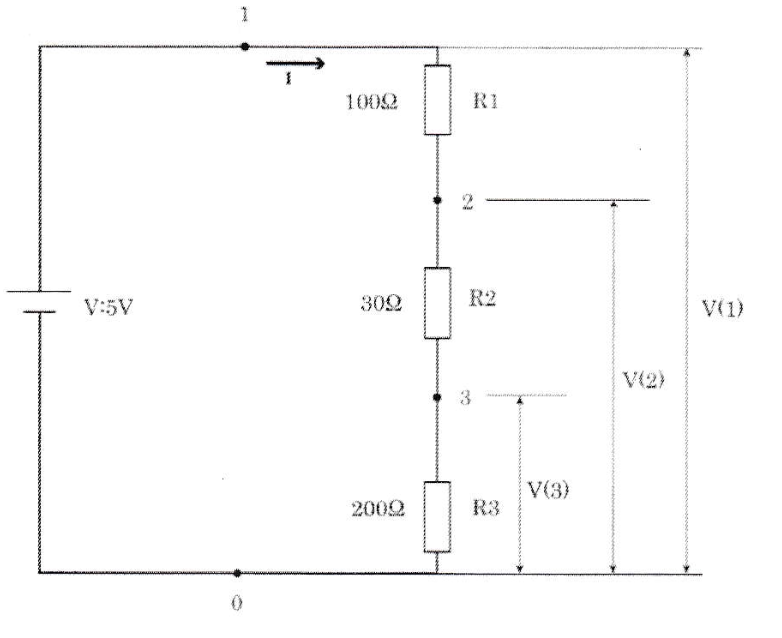
\includegraphics[width=0.6\textwidth]{assets/yobiex.png}
  \caption{予備実験回路}
\end{figure}

\begin{table}[H]
  \centering
  \caption{実験結果の比較}
  \begin{tabular}{|c|c|c|c|c|c|c|}
    \hline
    確認項目 & \( V(1) \) [V] & \( V(2) \) [V] & \( V(3) \) [V] & \( I \) [mA] & \( V_{12} \) & \( V_{23} \) \\ \hline
    実測値 & 5.00 & 3.48 & 3.05 & 14.17 & 1.52 & 0.43 \\ \hline
    シミュレーション結果 & 5.00 & 3.48 & 3.03 & 15.15 & 1.52 & 0.45 \\ \hline
    理論値(計算値) & 5.00 & 3.48 & 3.03 & 15.15 & 1.52 & 0.45 \\ \hline
    誤差率(%) & 0.00 & 0.00 & 0.6 & 0.0 & 0.0 & 4.4 \\ \hline
  \end{tabular}
\end{table}

\subsection{線形抵抗回路解析}
図3.2に示した回路を構築し、付録に記載したネットリストを用いてSPICEでシミュレーションを実行した結果を基に、表3.2を作成した。

\begin{figure}[H]
  \centering
  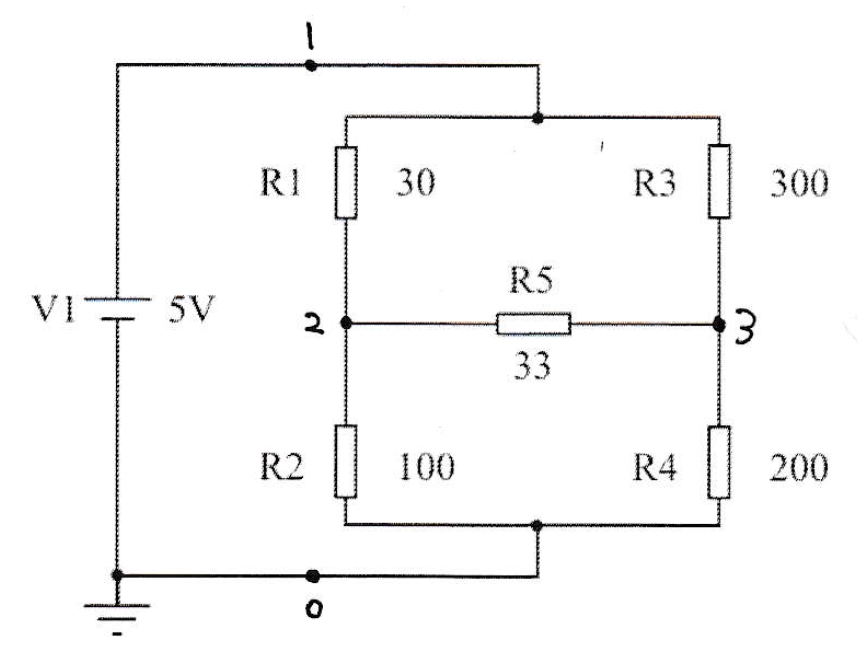
\includegraphics[width=0.6\textwidth]{assets/senkeikairo.png}
  \caption{線形抵抗回路}
\end{figure}

\begin{table}[H]
  \centering
  \caption{実験結果の比較}
  \begin{tabular}{|c|c|c|c|c|}
    \hline
    確認項目 & \( V(1) \) [V] & \( V(2) \) [V] & \( V(3) \) [V] & \( I \) [mA] \\ \hline
    実測値 & 5.00 & 3.53 & 3.23 & 45.4 \\ \hline
    シミュレーション結果 & 5.00 & 3.60 & 3.26 & 52.3 \\ \hline
    誤差率(%) & 0.0 & 1.9 & 0.9 & 13.2 \\ \hline
  \end{tabular}
\end{table}

\subsection{非線形抵抗回路解析}
図3.3に示した回路を構築し、付録に記載したネットリストを用いてSPICEでシミュレーションを実行した結果を基に、表3.3を作成した。

\begin{figure}[H]
  \centering
  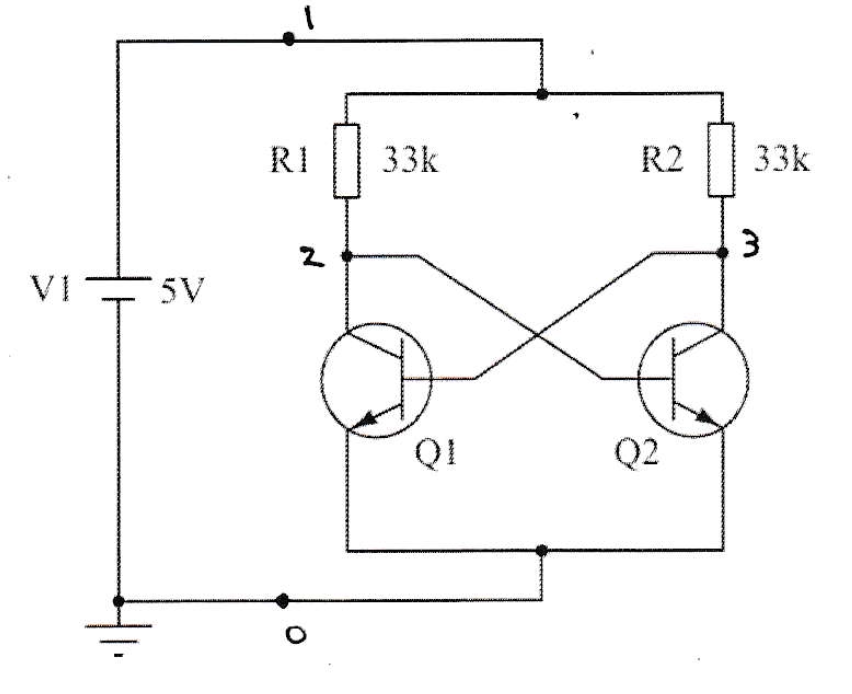
\includegraphics[width=0.6\textwidth]{assets/hisenkeikairo.png}
  \caption{非線形抵抗回路}
\end{figure}

\begin{table}[H]
  \centering
  \caption{実験結果の比較}
  \begin{tabular}{|c|c|c|c|c|}
    \hline
    確認項目 & \( V(1) \) [V] & \( V(2) \) [V] & \( V(3) \) [V] & \( I \) [mA] \\ \hline
    実測値 & 5.00 & 0.645 & 0.017 & 0.27 \\ \hline
    シミュレーション結果 & 5.00 & 0.603 & 0.603 & 0.267\\ \hline
    誤差率(%) & 0.0 & 6.97 & 97.2 & 1.1 \\ \hline
  \end{tabular}
\end{table}

\subsection{DC解析}
図3.4に示した回路を作成し、V2の電圧を0.1Vから5.0Vまで変化させたときの電流Iを測定することで表3.4を作成した。また、付録に記載したネットリストを用いてSPICEでシミュレーションを実行し作成したグラフを図3.5に示す。

\begin{figure}[H]
  \centering
  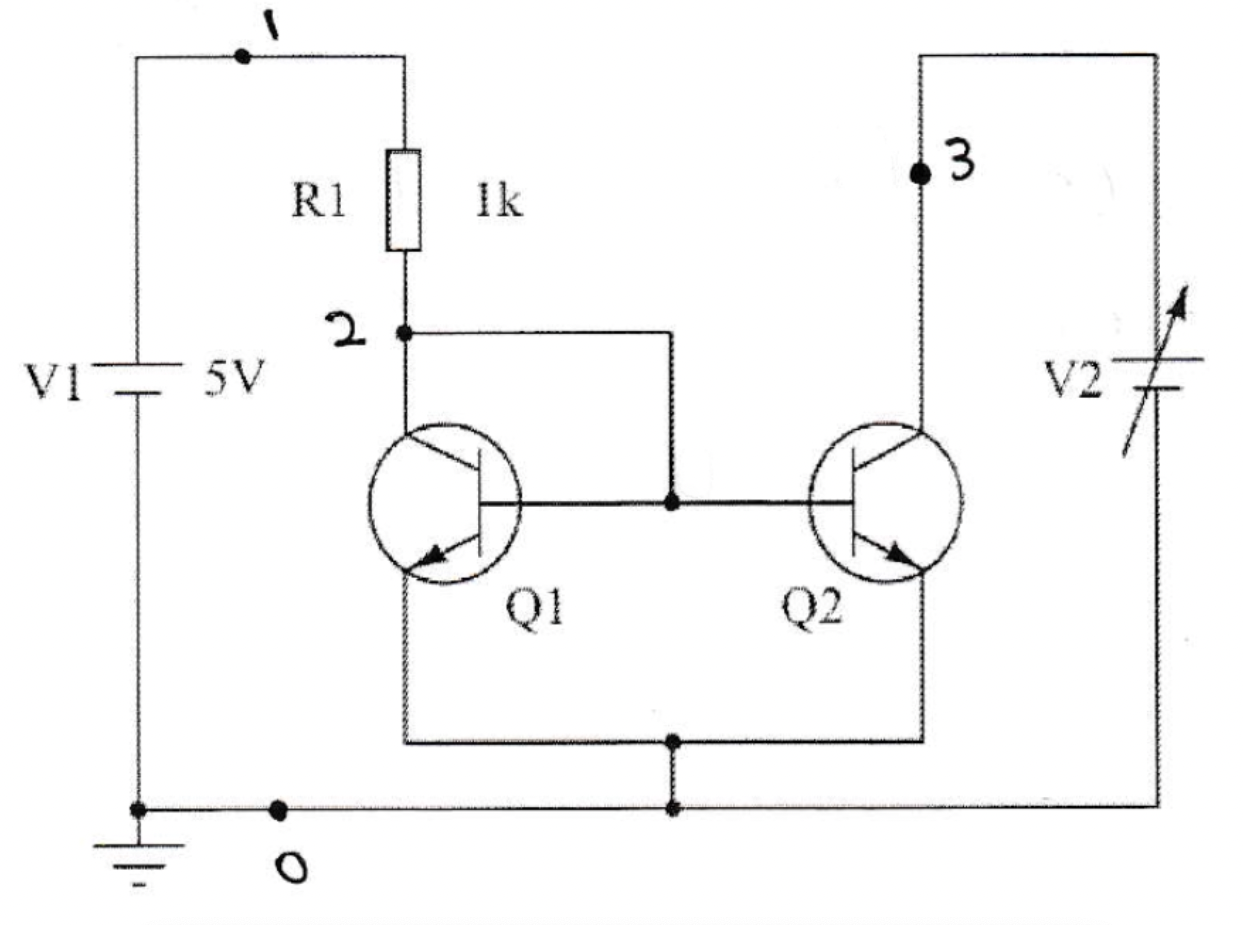
\includegraphics[width=0.6\textwidth]{assets/dckairo.png}
  \caption{DC解析回路}
\end{figure}

\begin{table}[H]
  \centering
  \caption{実験結果}
  \begin{tabular}{|c|c|}
    \hline
    \( V_{2} \) [V] & \( I\) [mA] \\ \hline
    0.1 & 4.08 \\ \hline
    0.2 & 4.08 \\ \hline
    0.4 & 4.08 \\ \hline
    0.6 & 4.08 \\ \hline
    0.8 & 4.08 \\ \hline
    1.0 & 4.08 \\ \hline
    2.0 & 4.09 \\ \hline
    3.0 & 4.09 \\ \hline
    4.0 & 4.10 \\ \hline
    5.0 & 4.10 \\ \hline
  \end{tabular}
\end{table}

\begin{figure}[H]
  \centering
  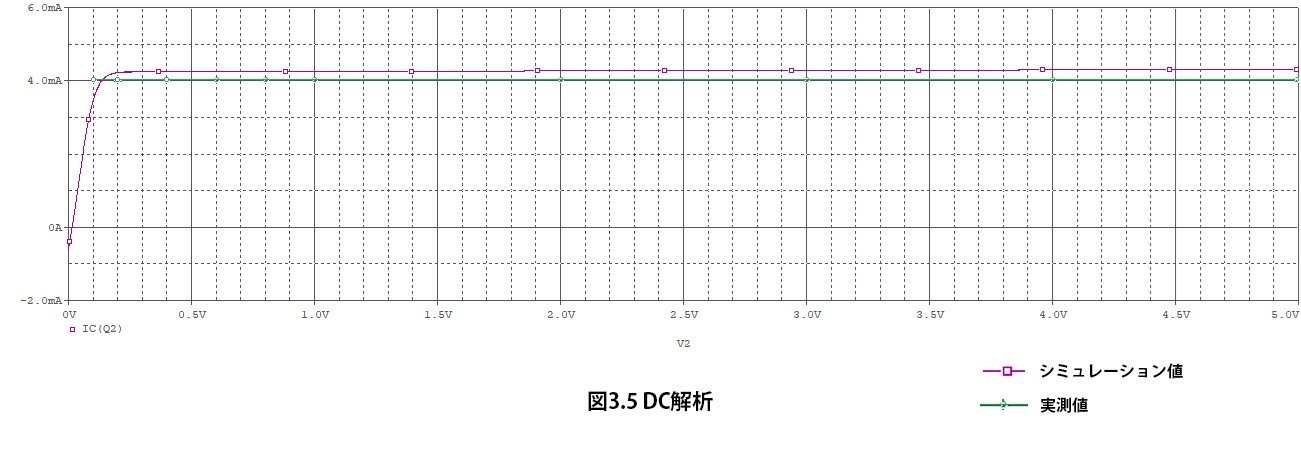
\includegraphics[width=\textwidth]{assets/dckaisekiplot.png}
  \caption{DC解析}
\end{figure}

\subsection{AC解析}
図3.6に示した回路を作成し、V1の周波数を20Hzから100kHzまで変化させたときのノード4(Vout)の電圧を測定した結果をもとに表3.5を作成した。また、付録に記載したネットリストを用いてSPICEでシミュレーションを実行し、さらに実測値をプロットし作成したグラフを図3.7に示す。

\begin{figure}[H]
  \centering
  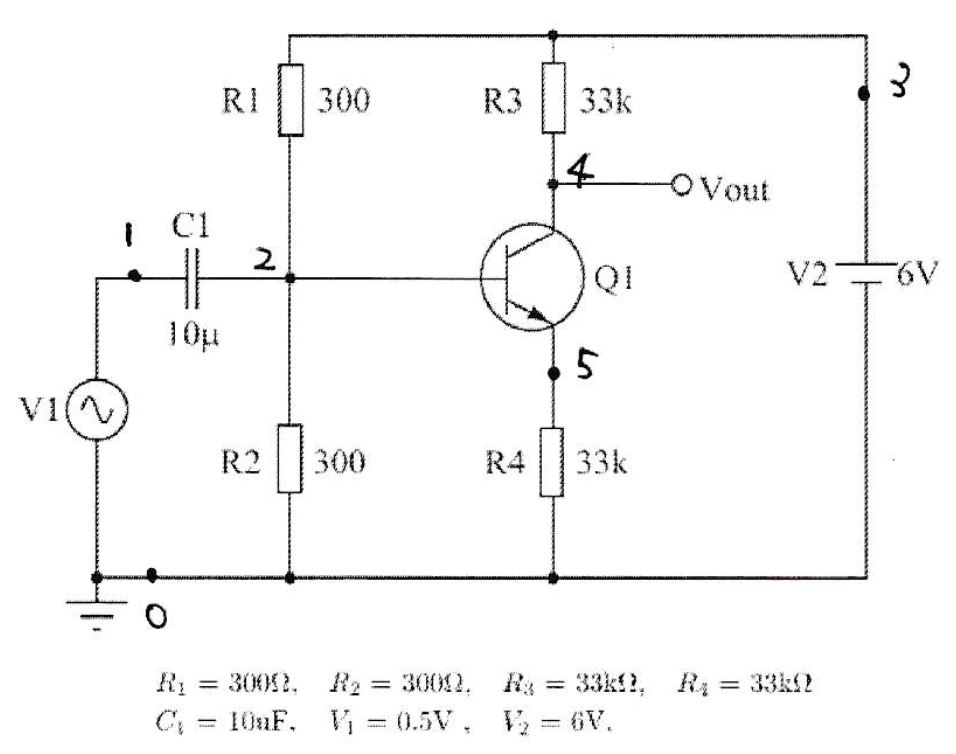
\includegraphics[width=0.7\textwidth]{assets/ackaisekikairo.png}
  \caption{AC解析回路}
\end{figure}

\begin{table}[H]
  \centering
  \caption{AC解析結果}
  \begin{tabular}{|c|c|}
    \hline
    周波数 [Hz] & 電圧 [mV] \\ \hline
    20 & 400 \\ \hline
    30 & 400 \\ \hline
    100 & 600 \\ \hline
    300 & 600 \\ \hline
    1k & 600 \\ \hline
    3k & 1000 \\ \hline
    10k & 1000 \\ \hline
    30k & 1000 \\ \hline
    100k & 1000 \\ \hline
  \end{tabular}
\end{table}

\begin{figure}[H]
  \centering
  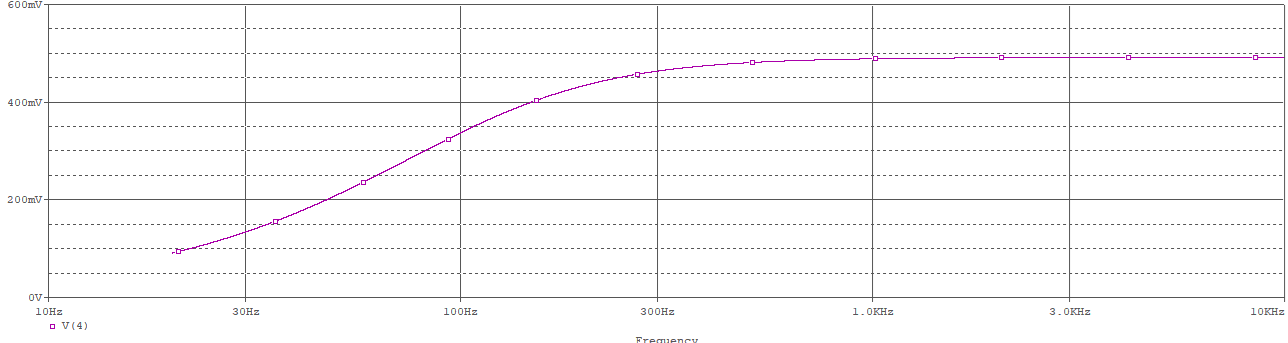
\includegraphics[width=\textwidth]{assets/ackaisekiplot.png}
  \caption{過渡解析}
\end{figure}

\subsection{過渡解析}
図3.8に示した回路を作成し、ノード2(V)の電圧を測定した結果をもとに表3.6を作成した。オシロスコープでの観測波形を図3.8に示す。なお、周期のはじまりの電位を0V基準かつ時刻t=0とし、そこからのΔVの値を記録した。また、付録に記載したネットリストを用いてSPICEでシミュレーションを実行し、さらに実測値をプロットし作成したグラフを図3.9に示す。

\begin{figure}[H]
  \centering
  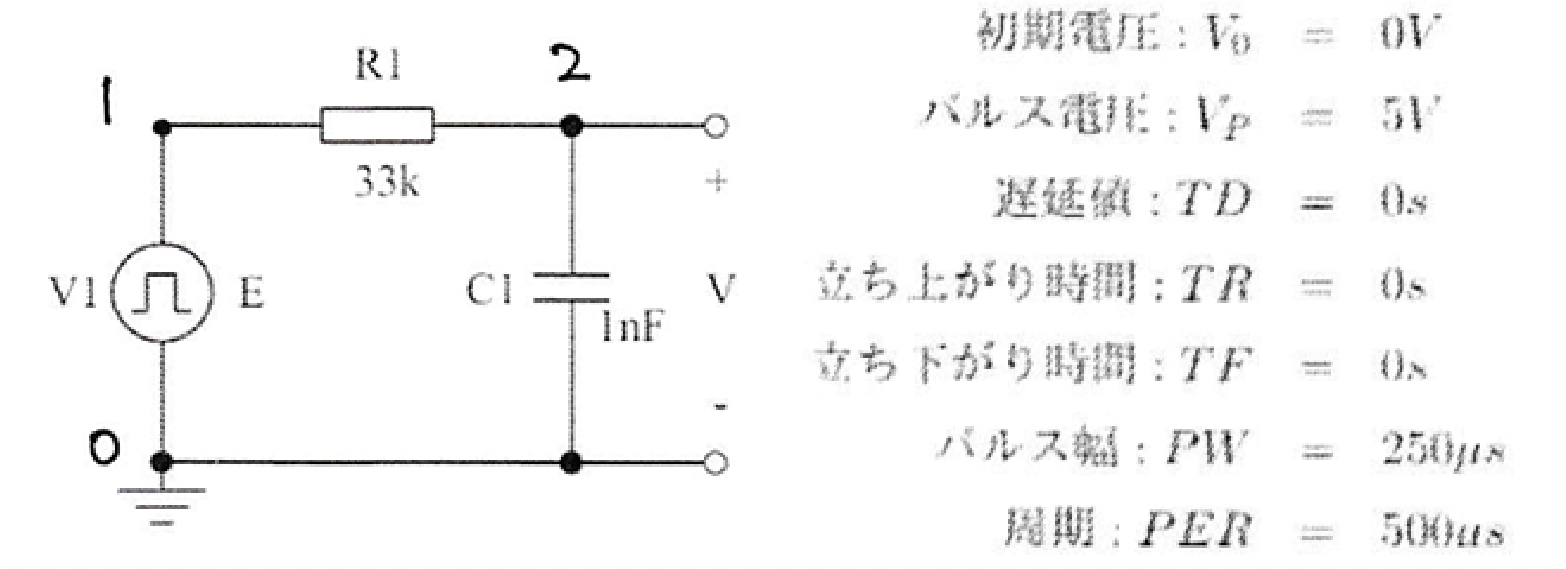
\includegraphics[width=0.8\textwidth]{assets/katokaisekikairo.png}
  \caption{過渡解析回路}
\end{figure}

\begin{table}[H]
  \centering
  \caption{過渡解析結果}
  \begin{tabular}{|c|c|}
    \hline
    \( t \) [\(\mu\)s] & \( V \) [V] \\ \hline
    0 & 0 \\ \hline
    50 & 3.84 \\ \hline
    100 & 4.64 \\ \hline
    150 & 4.72 \\ \hline
    200 & 5.04 \\ \hline
    250 & 5.12 \\ \hline
    300 & 1.12 \\ \hline
    360 & 0.32 \\ \hline
    400 & 0.08 \\ \hline
  \end{tabular}
\end{table}

\begin{figure}[H]
  \centering
  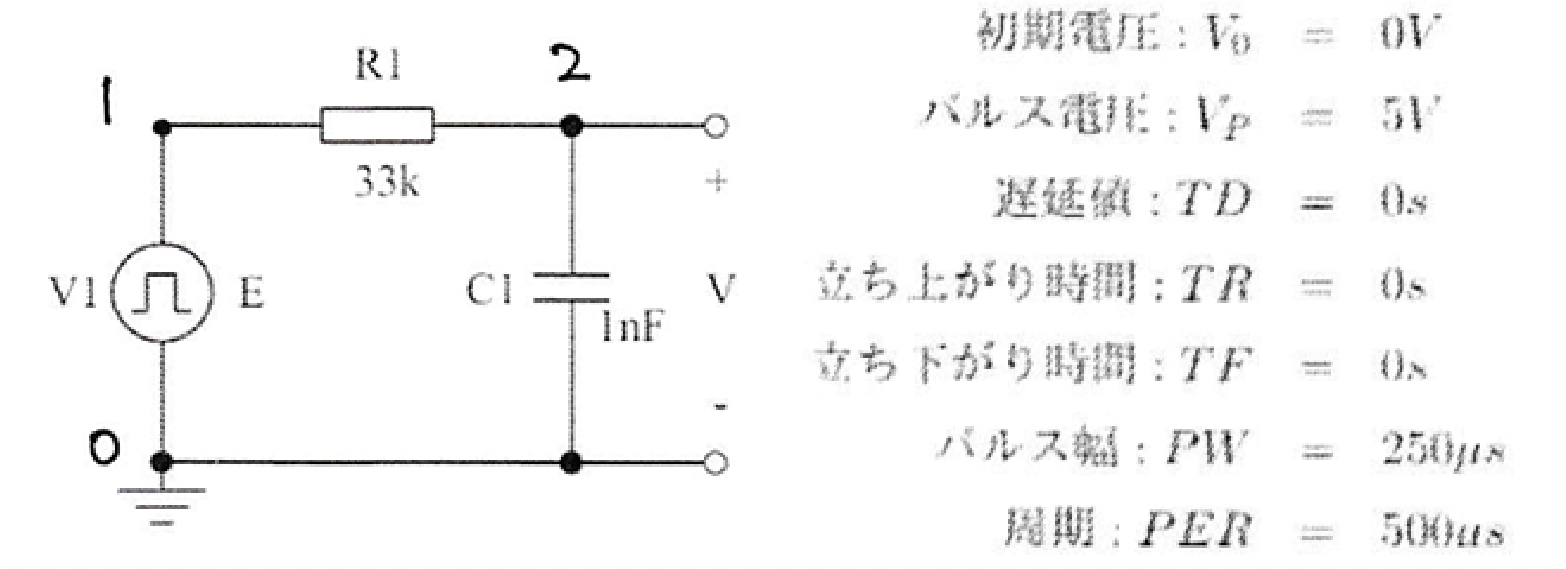
\includegraphics[width=0.8\textwidth]{assets/katokaisekikairo.png}
  \caption{オシロスコープでの観測波形}
\end{figure}

\begin{figure}[H]
  \centering
  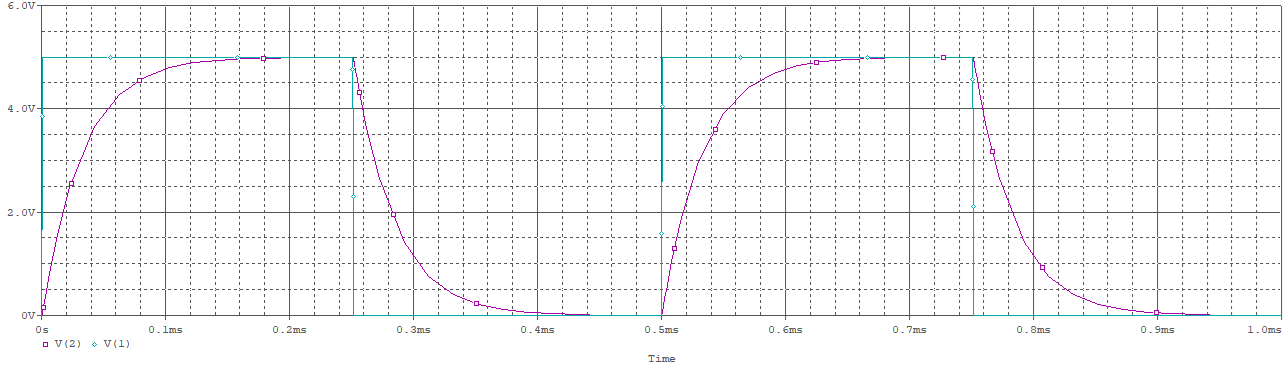
\includegraphics[width=\textwidth]{assets/katokaisekiplot.png}
  \caption{過渡解析}
\end{figure}

\section{使用機材}

\section{参考文献}
\begin{enumerate}
  \item SPICEとは, 電子回路シミュレーションの基礎 \\
    \url{https://techweb.rohm.co.jp/product/simulation/7688/}\\
    閲覧日:2025年5月17日
  \item アナログ電子回路シミュレータのメリット・デメリット \\
    \url{https://spiceman.jp/circuit-simulator-merit-demerit/}\\
    閲覧日:2025年5月17日
  \item 長尾佑紀, 『数値計算の常識を変える! 安定性で選ぶ常微分方程式の数値解法』, 共立出版, 2022年.
\end{enumerate}

\section{付録}
本実験のシミュレーションで使用したSPICEのネットリストを以下に示す。
\subsection{線形抵抗回路解析}

\subsection{非線形抵抗回路解析}

\subsection{DC解析}

\subsection{AC解析}

\subsection{過渡解析}

\end{document}